\documentclass[onecolumn, draftclsnofoot,10pt, compsoc]{IEEEtran}
\usepackage{graphicx}
\usepackage{url}
\usepackage{setspace}
\usepackage{pdfpages}
\usepackage{lscape}

\usepackage{geometry}
\geometry{textheight=9.5in, textwidth=7in}

% 1. Fill in these details
\def \CapstoneTeamName{		Project BoxSand}
\def \CapstoneTeamNumber{		6}
\def \GroupMemberOne{			Max Moulds}
\def \GroupMemberTwo{			Sam Morey}
\def \GroupMemberThree{			Anya Lehman}
\def \CapstoneProjectName{		Project BoxSand}
\def \CapstoneSponsorCompany{	Oregon State Physics Department}
\def \CapstoneSponsorPerson{		Dr. Kenneth Walsh}

% 2. Uncomment the appropriate line below so that the document type works
\def \DocType{		Problem Requirements
				%Requirements Document
				%Technology Review
				%Design Document
				%Progress Report
				}
			
\newcommand{\NameSigPair}[1]{\par
\makebox[2.75in][r]{#1} \hfil 	\makebox[3.25in]{\makebox[2.25in]{\hrulefill} \hfill		\makebox[.75in]{\hrulefill}}
\par\vspace{-12pt} \textit{\tiny\noindent
\makebox[2.75in]{} \hfil		\makebox[3.25in]{\makebox[2.25in][r]{Signature} \hfill	\makebox[.75in][r]{Date}}}}
% 3. If the document is not to be signed, uncomment the RENEWcommand below
%\renewcommand{\NameSigPair}[1]{#1}

%%%%%%%%%%%%%%%%%%%%%%%%%%%%%%%%%%%%%%%
\begin{document}
\begin{titlepage}
    \pagenumbering{gobble}
    \begin{singlespace}
        \hfill 
        % 4. If you have a logo, use this includegraphics command to put it on the coversheet.
        %\includegraphics[height=4cm]{CompanyLogo}   
        \par\vspace{.2in}
        \centering
        \scshape{
            \huge CS Capstone \DocType \par
            {\large\today}\par
            \vspace{.5in}
            \textbf{\Huge\CapstoneProjectName}\par
            \vfill
            {\large Prepared for}\par
            \Huge \CapstoneSponsorCompany\par
            \vspace{5pt}
            {\Large\NameSigPair{\CapstoneSponsorPerson}\par}
            {\large Prepared by }\par
            Group\CapstoneTeamNumber\par
            % 5. comment out the line below this one if you do not wish to name your team
            \CapstoneTeamName\par 
            \vspace{5pt}
            {\Large
                \NameSigPair{\GroupMemberOne}\par
                \NameSigPair{\GroupMemberTwo}\par
                \NameSigPair{\GroupMemberThree}\par
            }
            \vspace{20pt}
        }

    \end{singlespace}
\end{titlepage}
\newpage
\pagenumbering{arabic}
\tableofcontents
% 7. uncomment this (if applicable). Consider adding a page break.
%\listoffigures
%\listoftables
\clearpage

% 8. now you write!

\section{Introduction}
This document defines the goals and requirements of the 2017-2018 Project BoxSand development team. Since this is the first large-scale overhaul to the BoxSand project, this development team should focus specific client requirements for this development cycle while also developing long-term and overarching development goals and procedures for future project development.

\subsection{Purpose}
The purpose of this document is to describe the requirements for the 2017-2018 Project BoxSand development team and to document future features and functionality. The development team will also create an initial proof-of-concept for application functionality demonstration and enumerate the future features as requested by the client. For this cycle of development, this development team will complete the following specific goals for new functionality:
\begin{enumerate}
    \item The site that will be developed must provide access to the OpenStax Physics textbook within the site itself
    \item Provide a homework system within the site that allows an instructor of a course to provide questions with answers, Assign a value to the question and, assign a group of questions or a single question as an assignment to a course.
    \item Instructor must also be able to assign reading homework from the textbook for students within a course
    \item An instructor must be able to download a gradebook of student scores
\end{enumerate}


\subsection{Scope}
The scope of this document is to define the goals of this development cycle and a corresponding development team operating during the 2017-2018 Project BoxSand development cycle. This document will also serve as a the starting point for the next cycle of development of BoxSand.



\subsection{Definitions, Acronyms, and Abbreviations}
In this document the term application is used to refer to the work product being produced by the development team. Furthermore, the application has two underlying aspects depending on the context of the entity using the application and are referred to as the site, if the context is the user, or the system or server, if the context is the developer. Occasionally the two are used interchangeably. Additionally, BoxSand and Project BoxSand refer to the same entity, as does client and customer. The OpenStax framework is sometimes referred to as just the framework, or as a software component. The development team, or team,  is the term used to describe the group carrying out the work defined in this SRS and occasionally referred to as “we” in this and other documents referenced by this document. Below are a list of some less common terms and definitions. 

\subsubsection{Adaptive Learning}
Adaptive learning is a term used to describe a feature of a learning management system that is capable of using student performance data on a set of assessments to change how those assessments are presented, worded, or grouped in an effort to increase student success. 

\subsubsection{AsyncSync}
AsyncSync is a codename for the next set of features for BoxSand and specifically pertains to feature sets that have adaptive learning elements and improve features that foster peer-to-peer interaction. (See the BoxSand Milestone and Component Roadmap documents for more information on AsyncSync features.)

\subsubsection{CAS}
CAS stands for Central Authentication Service and provides authentication services for members of the OSU campuses. 

\subsubsection{COSINe}
COSINe is the name of a division of the of Arts and Sciences at OSU and provides IT support and assistance to the Physics department and have been maintaining the existing BoxSand site.

\subsubsection{Daily Learning Guide}
The daily learning guide is listing of resources created by an instructor to help guide student progression through course material and is currently used in the existing BoxSand site. This functionality will be translated to the new application by the development team.

\subsubsection{OER}
OER is an acronym for Open Educational Resource and has various similar working definitions. One definition that is often cited is the William and Flora Hewlett Foundation definition which defines OER as:
\begin{quote}
teaching, learning, and research resources that reside in the public domain or have been released under an intellectual property license that permits their free use and re-purposing by others. Open educational resources include full courses, course materials, modules, textbooks, streaming videos, tests, software, and any other tools, materials, or techniques used to support access to knowledge.[1]
\end{quote}

\subsection{References}
[1] "Open Educational Resources". The William and Flora Hewlett Foundation. 
www.hewlett.org/strategy/open-educational-resources. Retrieved 1 November 2017.

\subsection{Overview}
This document will continue to define the requirements of the 2017-2018 development cycle in the following two sections. This includes describing the features and functionality to be implemented in this cycle, described in section 2, and an overview of the requirements for those features, described in section 3. This project includes many forwarding looking features of which complete implementation is not required during this development cycle, planning and design considerations for these features has been included in this document and in the remaining sections. Requirements listed below that are beyond what was already listed in the purpose section above should not be considered explicit requirements as requested by the client.

Section 2 contains the user stories and roles along with the operations and functions performed by these requirements. This section also includes constraints and other requirements that are not immediately apparent. Additional documentation of these constraints will be ongoing and further described in future documents.

Section 3 expands on the requirements needed for the proposed solution from the Problem Statement and builds off of the feature descriptions in section 2. More information about specific technical aspects will be contained in future documentation including the Technical Review. 

\section{Overall Description}
This section describes the site generally as it would function to a user, detailing the non-functional requirements of the application. This section consists of a perspective detailing the motivation behind the relevant components, the interface to those components, and finally the operations performed by those functions with respect to the site. See section 3 for the descriptions of the requirements for the system aspect of the application.


\subsection{Product Perspective}
The application consists of two main parts. One part is the site and its accompanying framework used to display the second part, which is the content. For this development cycle the team will be using only a subset of the possible content to develop the application.

\subsubsection{User Interfaces}
The BoxSand project interacts with users through modern web browsers. From a web browser a user will be able to interact with the site and use the components described below: 
\begin{enumerate}
\item Landing page: Where a non signed in user will be directed upon arriving at the BoxSand website. This page will include a small about section and options to either login through ONID or visit as a guest.

\item Student User Dashboard: This page will show a registered user what they have accomplished in their course. It will include a small section for an optional profile picture and description. It will also show what learning modules the student has completed and the corresponding scores if any.

\item Instructor User Dashboard: This page will allow the instructor to view the content they have contributed for the course. Additionally the Instructor will be able to view assigned homework, and readings through this page.

\item Content pages: These pages will vary depending on what content is on the page. They will have a variation of: images, videos, textbook info, and homework depending on what the page will be showing. In general these pages will have a central area for the content and a section one the left hand side to show where the user is in the current module. 
\end{enumerate}

\subsubsection{Operations}
Users of the BoxSand site should be able to perform these operations:

\begin{enumerate}
\item A student will be able to :
\begin{enumerate}
\item Navigate the website through menus
\item Edit their personal profile (limited by standards compliance constraint)
\item Respond to homework questions
\item Interact with course content
\end{enumerate}
\item An instructor will be able to :
\begin{enumerate}
\item Navigate the site and course through menus
\item Edit the course, including:
\begin{enumerate}
    \item Editing (limited by constraint)
    \item Assign assessments
    \item View grades
\end{enumerate}
\end{enumerate}
\end{enumerate}

\subsubsection{Site Adaptation Requirements}
A process for transferring the content from the existing BoxSand site to the new application must be established and documented. Additionally, test content for one example lesson, course, and other related features that are to be developed must be included for the proof-of-concept demonstration. 

\subsection{Product Functions}
At the end of the development cycle these goals must be met:
\begin{enumerate}
\item Provide access to the OpenStax textbook and assessment library for BoxSand users.
\item A homework system that allows the instructor to add assessments to the course.
\item Ability for the instructor to assign assessments as homework or quizzes etc.
\item Ability for instructor to view the grades of students in a course 
\item Student dashboard for overview of the progress in course(s)
\item Instructor dashboard for overview of the progress of courses. 
\end{enumerate}

\subsection{User Characteristics}
There are two main types of users for the BoxSand site. One is the instructor or administrator, who will usually be a content author of some source of instructional content that serves as the core learning materials for a course. The other user is the student. Within the student user group, the type and role can be further broken down into registered and unregistered students. The registration mechanism discerning the two student types is detailed further in the Technical Review document and is administered by CAS.

\subsection{Constraints}

\subsubsection{Regulatory Policies}
The development team must be aware of FERPA and IRB requirements and adhere to those requirements for any final product. Additionally, the team should follow the best practices defined in the NIST Cybersecurity Framework. During development test data will provided that will not need to meet many of the requirements. (See Assumptions)

\subsubsection{Hardware Limitations}
The application must run on a hardware that is available to the development team. This is further specified in the technical review. This limitation could be relaxed by partnering with COSINe or OSU OSL. 

\subsubsection{Interfaces to Other Applications}
The site will interface with CAS, OpenStax, GitHub, and other services detailed in the Technical Review. During development these services will be used but for the final deployment the entire application must standalone and only interface with CAS. 

\subsubsection{Audit Functions}
The client need to be able to collect student site interaction data for the research project must be addressed by the development team. These will be available in a downloadable CSV file for the instructor. See previous documentation on the existing BoxSand site specifically about the export feature for more information. Log files from the site must also be generated in order to track student interaction and test site performance and where required by constraints and legal or partner requirements.

\subsubsection{Control Functions}
Control functions for the server will be collected and controlled by the container management suite that will be used. This is further specified in the Technical Review.

\subsubsection{Higher-order Language Requirements}
The site must be able to support future internationalization of the content but for this development cycle the immediate language requirement is English only. 

\subsubsection{Safety and Security Concerns}
Since the project will be using OSU’s CAS login system, the development team shall adhere to the security requirements imposed by that entity.

\subsection{Assumptions and Dependencies}
The team will assume that for this development cycle only one subject matter will be tested, Physics, and that content will be added from OpenStax and BoxSand only. Features and considerations for future content sources should be discussed and documented for future development.

The development team will have access to hardware and software needed to develop the OpenStax framework which is detailed on the OpenStax GitHub repositories. The team will also have access to a set of test content gathered from the BoxSand site content. 

\subsection{Apportioning of Requirements}
\begin{enumerate}
    \item Both reading from OpenStax textbook and from content on the BoxSand site
    \begin{enumerate}
        \item Reading assignments
        \item Video assignments
        \item Integrated questions with simulations
        \item Homework questions integrated with reading and videos
        \item Learning Modules can be created with due dates
        \item OpenStax Tutor Learning Module (LM) system, fully integrated with content and resources on the BoxSand.org site
    \end{enumerate}
    \item Ability to enter new questions and set up new forms of content in a user friendly interface
    \begin{enumerate}
        \item Multiple choice, numerical, free response, vector, ... etc.
        \item Ability to ask a range of question types
    \end{enumerate}
    \item Student Dashboards
    \begin{enumerate}
        \item Students can easily see what learning module they have completed and what they have left to do
        \item Statistics can be shown for average grade based on their particular web behavior
        \item Student facing dashboards
    \end{enumerate}
    \item Instructor Dashboards
    \begin{enumerate}
        \item See any one student's progress within the a course administered by that instructor
        \item See statistics on the aggregate student engagement for courses that instructor is associated with
    \end{enumerate}
    \item Ability to generate a downloadable CSV gradebook of student scores
    \item AsyncSync capabilities
    \begin{enumerate}
        \item Students will be automatically paired with students working on the same learning modules and provided shared chat channels and virtual whiteboard
        \item Be able to associate groups of students based on current progression through material
    \end{enumerate}
\end{enumerate}

\section{Specific Requirements}
As stated in the Problem Description, the development team will meet these goals:
\begin{enumerate}
\item Provide access to the OpenStax textbook.
\item Provide access and implement the OpenStax assessment library (eg. questions, quizzes etc)
\item Assign reading homework from the textbook
\item Provide exportable user tracking data used to study relationships between student interaction and performance. 
\end{enumerate}
More specifically, the development team must strive to meet these goals:
\begin{enumerate}
\item The website that will be developed must provide access to the OpenStax Physics textbook within the site itself. 
\item Users will be able to log in as either a student or as an instructor. If the user is a student then they will be able to:
\begin{enumerate}
    \item Log in using their school login. A current OSU student will be able to login using their ONID account. 
    \item See what has been assigned to them. All assigned assignments will be listed on the student’s dashboard so they can see them.
    \item Complete online homework. When logged in as a student, the user will be able to answer the assigned questions. 
    \item Access the online textbook and other provided resources. Content that is currently on the BoxSand site will be pulled into the new site.
\newline If the user is logged in as an Instructor then they will be able to:
    \item Login to a different view of the software from that of the students. A current OSU teacher will be able to login using their ONID account.
    \item Assign homework and reading to the students with due dates. An instructor user will be able to create an assignment by combining pieces of the BoxSand text and questions drawn from a bank of questions. Those assignments will have the ability to be given a due date.
    \item Add questions to the database of homework problems. An instructor will be able to submit a new question to the database of homework questions.
    \item An instructor will be able to download a CSV file of the students and the grades they got on their homework.
\end{enumerate}
\item Provide a homework system within the site that allows an instructor of a course to provide questions with answers, Assign a value to the question and, assign a group of questions or a single question as an assignment to a course.
\item Instructor must also be able to assign reading homework from the textbook for students within a course
\item An instructor must be able to generate a downloadable gradebook of student scores
\end{enumerate}

\subsection{External Interfaces}
This section describes inputs into and outputs from the application. It also gives a description of the hardware, software and communication interfaces and provides basic prototypes of the user interface.

\subsubsection{User Interface}
The development team will extend some of the functionality of the OpenStax platform to include user tracking and custom content. There will be a user interface that represents the content used within a course and will be closely related to the OpenStax framework and style of user interface in order to meet the software system criteria. Please refer to future documents detailing the wireframe for this interface.

\subsubsection{Hardware Interfaces}
There are no explicit hardware interfaces other than those traditionally required with web applications. A partnership with COSINe is being developed during the writing of this document. It has also been discussed that a final deployment of the application could reside on OSU OSL hardware. More information on this interface will be provided in future documents as it becomes available.  

\subsubsection{Software Interfaces}
The development team will interface with the upstream provider for the OpenStax framework through the GitHub service. The team will also develop the specific interface for the CAS login system for BoxSand.

\subsection{Functional Reqiurements}
This section describes elements of the functional requirements needed by the application. Both site and system requirements are described and more information on specific implementations can be found in the Technical Review and other project documents. 

\subsubsection{Login}
The system as defined by the client requirements must be able to verify user identities and accept or reject service requests through the site based on identity and group associations of that identity. This will be further defined in the Technical Review document and involves interfacing with CAS. 

\subsubsection{Content Display}
The system will also provide the required software dependencies for the framework as listed in the Technical Review document. This includes complete support of the client requirements as listed in the purpose section of this document..

\subsubsection{Homework System}
The system will also provide a site level functionality that allows instructors to group assessments into other graded assessments and assign that new assessment to a course, student or group of students. 

\subsubsection{Dashboard}
The system must support the site feature of dashboards for all user types and correctly display data based on user association(s) with the site. This includes displaying elements of the user tracking reports mentioned later in this document of specific user roles where allowed by IRB and FERPA restrictions. 

\subsubsection{User Tracking}
The site must track user interaction with the site and communicate that information with the system. The information that is tracked is listed in the BoxSand User Tracking document and at a minimum mirrors the information tracked by the old BoxSand site user tracking tools. 

\subsubsection{Tracking Report}
The system will be capable of generating a grade report for registered users of a course for an instructor or an administrator and be able to create reports for unregistered and registered users for administrators. This depends on the previous requirement.

\subsection{Performance Requirements}
The client has stated that all functions of the new application that are present in the old site should be performed in equal or less time than on the old site. This includes all functionality during peak usage and worst case scenario situations. To meet this requirement the development team must analyze the existing site to determine the those parameters. The new application must also support the same number of user at deployment. (See the non-functional requirement for scalability)

\subsection{Logical Database Requirements}
The format and specific fields for the database containing all the user tracking data is still being actively discussed but mostly contains data relating to a activity of a user on the site and will not contain grade or personally identifiable information in that database. When grade information is needed, it must be stored in a separate database and must be used in accordance with FERPA and other legal requirements. In addition to the constraints of that database, the development team may be required to provide an option to store grade data with another software interface called Canvas which is used at OSU as a basic learning management system. This option is partly implemented already in the OpenStax framework and is still actively being investigated. 

\subsection{Software System attributes}
The following section details fit criteria for the non-functional aspects of the application and underlying system and site. Since this section will also change slightly as the needs of the client change during the development cycle not all criteria are explained in detail here. 

Two major long-term goals driving this project are providing access to OERs and having all content and other required services all in one application. This means that site interaction must be limited to just this application and where possible certain non-functional criteria should be favored over others. 

\subsubsection{Usability and Effectiveness}
The development team is specifically tasked with integrating the usability of the existing BoxSand with new client requirements and the OpenStax framework, more or less. This implies that while future iterations of this application will have a large audience to which the engineered usability must be adjusted to, the immediate goal of this cycle is in success of this application meeting the current needs of the client. The ramification from this requirement is most evident in the constraint of the instructor dashboard feature set. It is also expected that during development some other features may be sacrificed for a more immediate usability. While usability is not solely contributing the applications effectiveness, it is a large portion.

\subsubsection{Reliability}
The system must maintain a reliable interface with the outside world. This includes correctly identifying and reporting application status to users and the application should not allow a user to interact with a system component that is not fully functional. Also, special consideration should be given to data integrity of the research data collection components.

\subsubsection{Extensibility and Scalability}
These two non-functional requirements have similar levels of importance and required adherence in this development cycle. The OpenStax framework is being brought into this project as a software source to develop a greater level of extensibility, scalability and maintainability. As the need to support a defined number of users is still a variable at the time this document was written stating that the new application should be able to scale to a level capable of providing the application to the existing BoxSand user base without service degradation. Further information on this as a functional requirement will be described in the Technical Review document.

\subsubsection{Interoperability}
The application uses component provided by other software sources, such as OpenStax. Where possible, a best effort should be maintained throughout the development cycle to keep the OpenStax framework used by the BoxSand application as close to the current OpenStax codebase as possible. This also applies to other software sources needed for the application. 

\subsubsection{Availability}
The deployed system must be able to maintain an uptime of 95% over an academic quarter. 

\subsubsection{Maintainability}
While the future maintenance of the application is not explicitly defined by the client, the client has strongly expressed a desire for future development and maintenance beyond the scope of this development cycle. All development processes such as documentation, discussion, testing, etc should be completed in such a way that another development team can continue process. 

\subsubsection{Portability}
This system will be designed for any part of the OSU curriculum but the deployed version will be tailored to the needs of the client. If time permits extending portability could be addressed but for this cycle the only concern for the development team during deployment is the immediate needs of the customer.

\subsubsection{Integrity, Testability, and Privacy}
The application should make an effort to report non-functional conditions and not allow operation during conditions of partial functionality. The application should also not release untested features of functionality and ensure that the research data generated from the application is as continuous  as possible during deployed operation. Concerning the testability of the application and underlying system, a best effort must be made to ensure industry best practices are followed that exceed minimum requirements set by all software partners. This is most important in regards to CAS and privacy concerns detailed in FERPA and IRB requirements. 

\subsubsection{Accessibility}
Future development cycles will address the accessibility of the application explicitly. For this reason, this development cycle is focused on proof-of-concept and initial development and therefore any  design around this criteria should be secondary except in areas where access is required by law. (See expanded constraint section in the Technical Review and future documentation)


\subsection{Appendixes}

\subsubsection{Appendix A - Gantt Chart (Continued on next page)}
\newpage
\begin{landscape}
\begin{figure}
 \centering 
  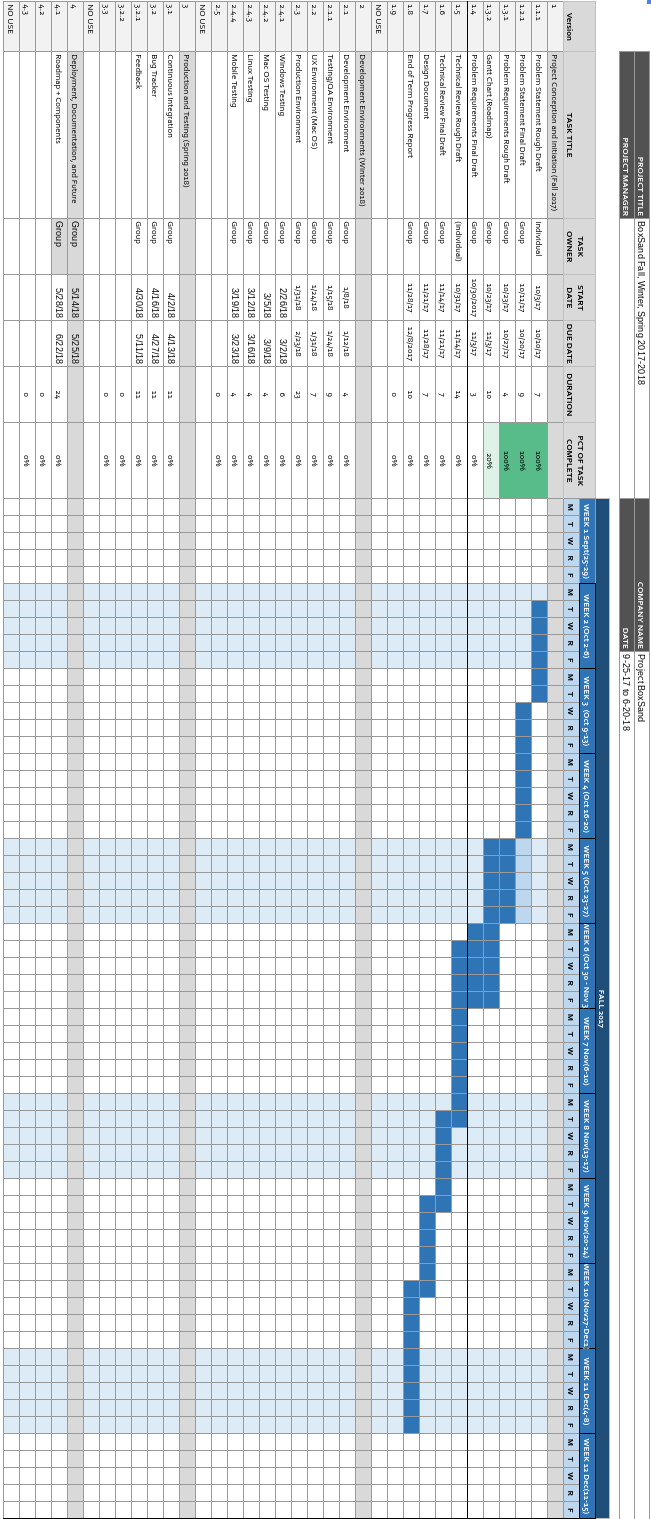
\includegraphics[angle=-90,width=\textwidth]{gantt.png}
\end{figure}
\end{landscape}
\end{document}
